\chapter{Pretrained Language Models}\label{ch:llm}

The meta-trained networks learn description statistics from repeated tasks. We next ask whether pretrained language models use the same information when it is stated explicitly. We use numerical mean estimation, a scalar version of the regression problem with fixed input $x=1$, following controlled tests of stated priors and in-context evidence \citep{gupta2025,akata2026}.

\section{Task and Evaluation}\label{sec:llm-task}

Each task has a hidden mean $w\sim\mathcal{N}(500,100^2)$ and demonstrations drawn from $\mathcal{N}(w,\sigma^2)$, with $\sigma=60$, then rounded to integers. A description supplies a value $m$ and uncertainty $\tau$, for example: ``Its mean was drawn from a normal distribution with mean 510 and standard deviation 30.'' The underlying Gaussian construction has $w\mid m\sim\mathcal{N}(m,\tau^2)$. We express precision in demonstration units as $c=\sigma^2/\tau^2$: stated standard deviations $60$, $30$, and $10$ correspond to $c=1$, $4$, and $36$.

We vary the stated precision, and add conditions stating a $50\%$ probability that the description is wrong. In these conditions the description remains relevant; the intervention tests how models respond to the stated probability. We also hold $m$ and the demonstrations fixed while describing a value generated at $c=36$ as having $c=4$. This isolates sensitivity to the stated uncertainty from sensitivity to the numerical value itself. Section~\ref{sec:llm-unreliability} includes genuinely irrelevant descriptions and evaluations under actual mixtures of relevant and irrelevant descriptions.

The main comparison uses the same $200$ tasks for five models with reasoning enabled and disabled: gpt-oss-20b \citep{openai2025}, Qwen3.5 9B \citep{qwen35}, Gemma~4 31B \citep{gemma4}, GPT-6 Sol, and Claude Opus~4.6. Claude Haiku~5.5 is evaluated with reasoning at medium effort. Checkpoints are held fixed within model, although serving environments and decoding settings differ for some comparisons. Sections~\ref{app:llm}--\ref{sec:llm-runs} report these details, response extraction, token limits, reruns, and a larger non-reasoning evaluation on $2{,}000$ tasks.

\paragraph{A reference based on the prompt.}
The prompt specifies the observation noise and description, but not the task generator's baseline prior. Our \emph{prompt-based Bayesian reference} therefore uses the stated description and a uniform fallback over the three-digit range. For a description asserted to be relevant, ignoring negligible boundary effects, its prediction is
\begin{equation}\label{eq:scalar-rule}
\hat w_{\mathrm{ref}}=\frac{c\,m+n\bar y}{c+n},
\end{equation}
where $\bar y$ is the demonstration mean. Under the continuous, correctly specified Gaussian model with a flat baseline prior, the description has exact ESS $c$. There is no random-design dimension term because every observation measures the same scalar mean.

Intuitively, the description counts as $c$ further demonstrations at $m$: it adds a precision of $1/\tau^2=c/\sigma^2$, equal to that of $c$ demonstrations. This is the conjugate normal model of Chapter~\ref{ch:background} with $n_0=c$, and the squared error is $\sigma^2/(c+n)$ with the description and $\sigma^2/n$ without it.

This reference follows the prompt even when a stated precision or reliability differs from the data generator. It is therefore a model of inference from the stated information, rather than an oracle for every evaluation condition. When the description may be wrong, its posterior also depends on the chosen fallback; we report sensitivity to that choice.

For each model, we compute ESS from its own demonstrations-only curve and summarize it by the median over $n\in\{1,2,4\}$. The same calculation gives reference ESS $34.6$ for $c=36$, rather than the idealized value $36$, because of finite-sample error and interpolation. We also regress predictions on $m$, $\bar y$, and an intercept. The coefficient on $m$ measures reliance on the description; the reference coefficient is $c/(c+n)$ when the description is asserted to be relevant.

\begin{figure}[htbp]
\centering
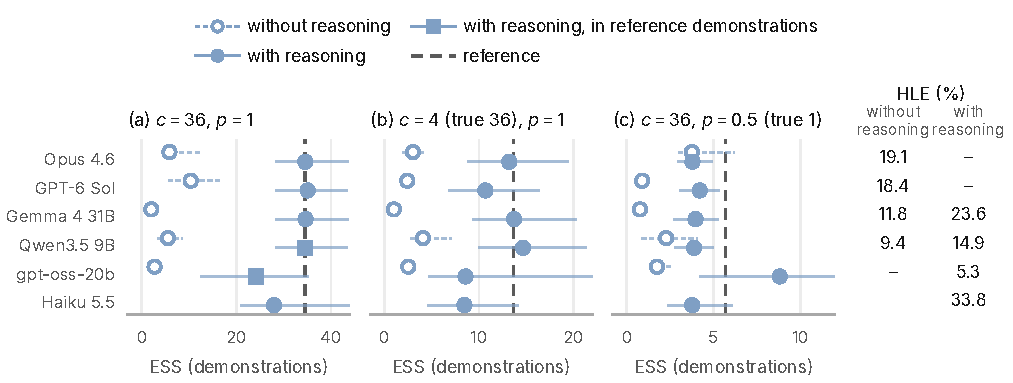
\includegraphics[width=\textwidth]{llm_ess.pdf}
\caption[Reasoning improves the use of stated precision, with model-specific exceptions]{\textbf{Reasoning improves the use of stated precision, with model-specific exceptions.} Summary ESS on $200$ tasks at $\sigma=60$: median over $n=1,2,4$, with paired $95\%$ bootstrap intervals over tasks. Open and filled points denote reasoning disabled and enabled; dashed and solid intervals distinguish the modes. Vertical dashed lines show the prompt-based Bayesian reference. (a) Relevant description with $c=36$: reference ESS $34.6$. (b) The same value, generated at $c=36$, is stated to have $c=4$: reference ESS $13.7$, because the value is more accurate than stated. (c) The description in (a) is assigned a $50\%$ probability of being wrong, while remaining relevant: reference ESS $5.7$ under the uniform fallback, which the prompt does not state. For GPT-6 Sol and Haiku~5.5, stating it changes which rule they follow but barely changes their ESS (Section~\ref{sec:llm-rules}). Square reasoning markers for Qwen3.5 9B in (a,b) and gpt-oss-20b in (a) use the reference's demonstrations-only curve because the models' own curves do not reach the crossing; these values are in reference-demonstration units. Haiku~5.5 uses medium effort. Intervals are clipped to the displayed range. HLE scores \citep{phan2025}, as reported by \citet{aa2026}, provide descriptive context; dashes indicate unavailable scores for the evaluated mode, and blanks indicate modes not evaluated.}
\label{fig:llm}
\end{figure}

\section{Reasoning and Stated Precision}\label{sec:once}\label{sec:reasoning}

\paragraph{Weak sensitivity without reasoning.}
For the $c=36$ description, non-reasoning ESS ranges from $1.5$ to $5.8$ across the five models, compared with $34.6$ for the reference (Figure~\ref{fig:llm}a). Models generally underweight this precise description and respond weakly when its stated precision changes. At $n=4$, GPT-6 Sol assigns weights $0.12$ and $0.13$ at stated $c=36$ and $c=4$, respectively, compared with reference weights $0.90$ and $0.50$. Opus~4.6 responds more, with weights $0.40$ and $0.20$. When the same value is described as $c=4$ instead of $c=36$, reference ESS falls from $34.6$ to $13.7$, whereas no model's ESS changes by more than $2.8$ (Figure~\ref{fig:llm}b).

\paragraph{Reasoning recovers precision weighting in several models.}
With reasoning enabled, Opus~4.6, GPT-6 Sol, and Gemma~4 31B reach approximately the reference ESS in both precision conditions; Haiku~5.5 at medium effort comes close. Among diagnostically separated tasks at $n=4$, the weight implied by an individual reply is within $0.05$ of the reference weight in $95$--$100\%$ of these models' replies (Section~\ref{sec:llm-rules}). This supports a change in how the description and demonstrations are combined, beyond an improvement in aggregate error alone.

Qwen3.5 9B and gpt-oss-20b also approach the reference precision weights, but arithmetic errors complicate their ESS. Their demonstrations-only curves can rise at larger $n$, preventing a crossing within the evaluated grid. For these cases, square markers in Figure~\ref{fig:llm} report sample equivalence using the reference's demonstrations-only curve, a different quantity from learner-specific ESS. Errors with the description also reduce gpt-oss-20b's ESS in some conditions. Reported HLE scores do not order these behaviors: some higher-scoring non-reasoning models use precision less accurately than lower-scoring reasoning models. This comparison is descriptive and does not isolate the mechanism responsible for the difference.

\section{Stated Reliability and Wording}\label{sec:llm-stated}

\paragraph{Reasoning models update relevance when the prompt says what a wrong description implies.}
Adding a stated $50\%$ probability of error lowers reference ESS from $34.6$ to $5.7$ under the uniform fallback. Without reasoning, no model's ESS falls by more than a factor of $2.7$, compared with a factor of about six for the reference. With reasoning, GPT-6 Sol, Gemma~4 31B, and Qwen3.5 9B closely track a different rule: they retain the stated relevance probability and weight $m$ by $p\,c/(c+n)$ (Table~\ref{tab:hedge}). This averages the relevant and irrelevant predictions using the \emph{prior} mixture weights.

Bayesian inference instead updates relevance by comparing how likely the demonstrations are if the description applies and if it does not. The prompt says only that the mean is then ``unknown'', which leaves the second likelihood, and so the update, undefined; keeping the stated probability is one defensible response. We therefore repeat the condition for GPT-6 Sol at low effort and Haiku~5.5 at medium effort, changing only the warning to say that the mean ``was instead drawn uniformly at random from the whole numbers 100 to 999'', the fallback the reference assumes. On tasks where the reference and fixed-rule predictions differ by at least $5$, the share of replies closer to the reference rises from $0$--$2\%$ to $89$--$97\%$ for GPT-6 Sol and from $21$--$41\%$ to $87$--$95\%$ for Haiku~5.5 (Section~\ref{sec:llm-rules}). Once the alternative is specified, both models update relevance from the demonstrations. The update is not always calibrated: with a stated $10\%$ chance, both rely on the description less than the reference does, and their ESS falls to about $18$, against $27.5$.

\paragraph{More explicit statistical descriptions are used more consistently.}
We test three alternative wordings with GPT-6 Sol and Haiku~5.5. Both closely follow Equation~\eqref{eq:scalar-rule} under the original wording and ``An earlier estimate put its mean at $m$, with a standard error of $\tau$.'' Under ``Its mean is about $m$, give or take $\tau$'' and ``Mean: $m\pm\tau$,'' they often return $m$ and disregard demonstrations. With the first informal wording, GPT-6 Sol skips reasoning in $24$--$51\%$ of replies per condition and usually returns $m$ in those replies. Haiku~5.5 returns $m$ in $71\%$ of the replies for which it does reason.

These alternatives preserve the numerical values but do not specify an equally precise statistical interpretation. The statistical wordings explain how the uncertainty should enter the task; informal uncertainty expressions leave that relationship less explicit. As with the unstated fallback, the finding therefore concerns the specificity of the description as a whole, including its instructions for interpreting uncertainty, rather than invariance to semantically equivalent phrasing.

\section{Additional Language-Model Results and Evaluation Details}\label{app:llm}

We generate $2{,}000$ tasks. Six open-weight models answer all tasks without reasoning; we refer to these experiments as the \emph{full run}. The models are gpt-oss-20b, Qwen3.5 9B, and Gemma~4 31B, which also appear in Sections~\ref{sec:llm-task}--\ref{sec:llm-stated}, together with Phi-4 (14B; \citealp{abdin2024}), OLMo~2 32B Instruct \citep{walsh2025}, and Gemma~4 12B. The experiments in Sections~\ref{sec:llm-task}--\ref{sec:llm-stated} use the first $200$ tasks. Unless stated otherwise, the results in this section and those that follow use the full run without reasoning.

Table~\ref{tab:llm} reports summary ESS, defined as the median over $n \in \{1,2,4\}$, with uncertainty intervals. Figure~\ref{fig:curves} shows the underlying learning curves. Tables~\ref{tab:llm-worth} and~\ref{tab:llm-worth-written}, in Appendix~\ref{app:llm-tables}, report ESS at every evaluated demonstration count; Table~\ref{tab:sensitivity} compares interpolation methods; Table~\ref{tab:llm-full}, also in Appendix~\ref{app:llm-tables}, reports description weights for the models with a distribution readout; and Table~\ref{tab:mixture} evaluates genuinely unreliable descriptions.

Throughout these sections, the \emph{prompt-based Bayesian reference} uses the probabilistic claims in the prompt together with an explicit assumption for the unspecified fallback prior. It is optimal under that assumed model. When the stated description differs from the data-generating process, it need not minimize error under the evaluation distribution. The reference labeled ``Bayes-optimal'' in the plots and tables has this meaning.

\section{Prompts, Tasks, and Model Readouts}

\paragraph{Model inclusion.}
We retain a model only if it produces a number in at least three quarters of replies overall and in at least half of replies without a description at each of $n = 1$, $2$, and $4$. The latter conditions determine the baseline curve used for summary ESS. This criterion excludes MiniCPM5~2B \citep{minicpm5}, OLMo~2 7B Instruct, and OLMo~2 13B Instruct, whose replies begin with a number in $62\%$, $20\%$, and $10\%$ of cases, respectively. These models often begin with explanations such as ``To predict\ldots'' or ``Given\ldots'' despite the numeric-only instruction. For example, OLMo~2 7B's summary ESS for the $c = 36$ description is $21$, but this value comes from a readout that rests on a minority of the model's probability.

The full run uses Hugging Face Transformers at each model's native precision, with checkpoints \nolinkurl{openai/gpt-oss-20b}, \nolinkurl{microsoft/phi-4}, \nolinkurl{allenai/OLMo-2-0325-32B-Instruct}, \nolinkurl{Qwen/Qwen3.5-9B}, \nolinkurl{google/gemma-4-12B-it}, and \nolinkurl{google/gemma-4-31B-it}. Tasks are sampled by a seeded generator. Reasoning is disabled where the chat template supports this option. For gpt-oss-20b, generation begins in the final channel, after the channel normally used for reasoning.

\paragraph{Distribution and written readouts.}
For gpt-oss-20b, Phi-4, and OLMo~2 32B without reasoning, the prediction is the mean of the first-token distribution over the $900$ three-digit number tokens. We call this the \emph{distribution readout}. These three models encode every three-digit integer as a single token, and we renormalize the first-token probabilities over these tokens. Other models, and all reasoning runs, use the number in the final answer, called the \emph{written readout}. We also evaluate written readouts for the three distribution-readout models as a robustness check (Tables~\ref{tab:llm} and~\ref{tab:paraphrase}). OLMo~2 32B assigns $41\%$ of first-token probability to numbers without a description at $n = 1$, and $75\%$ at $n = 2$. Its distribution readout at $n = 1$ therefore summarizes a minority of the first-token probability mass.

\begin{table}[htbp]
\centering\small
\setlength{\tabcolsep}{2.4pt}
\caption[Description ESS and weights in the full run without reasoning]{\textbf{Description ESS and weights in the full run without reasoning.} Left: median ESS over $n = 1$, $2$, and $4$, for relevant descriptions with $c = 1$, $4$, and $36$, and for the $c = 36$ description when irrelevant or accompanied by a stated $10\%$ or $50\%$ chance of being wrong. Brackets give $95\%$ bootstrap intervals. An upper bound, $\leq$, indicates that one demonstration alone outperforms the description-conditioned prediction. Right: the coefficient on the stated value at $n = 1$; the Bayesian reference weight is $c/(c+n)$. All results use $\sigma = 60$. ``Written'' denotes the written readout.}
\label{tab:llm}
\vspace{3pt}
\fittable{../../results/llm-test/llm_table.tex}
\end{table}

\paragraph{Prompt.}
The following text is supplied as the user turn in the model's chat template:
\begin{quote}\scriptsize\ttfamily\raggedright
The numbers below are drawn from a normal distribution with standard deviation 60.\\
Its mean was drawn from a normal distribution with mean 510 and standard deviation 30.\\[3pt]
548\\
431\\[3pt]
Predict the next number. Reply with the number only.
\end{quote}

Without a description, the second sentence is ``Its mean is unknown.'' To state unreliability, a third sentence is added: ``There is a 10\% chance that this statement is wrong, in which case the mean is unknown.'' In the rerun of Section~\ref{sec:llm-stated} that states the fallback, its last clause becomes ``in which case the mean was instead drawn uniformly at random from the whole numbers 100 to 999.'' With no demonstrations, the final question is ``Predict the first number.''

\paragraph{Task generation.}
A relevant description value is sampled conditional on the task so that the joint distribution satisfies $m \sim \mathcal{N}(500,100^2-\tau^2)$ and $w\mid m \sim \mathcal{N}(m,\tau^2)$. A task is redrawn if a displayed number or description value falls outside $100$ to $999$; this occurs for less than $1\%$ of tasks. The full run also includes $\sigma = 30$ conditions. Both standard deviations stated in the prompt are then halved, preserving $c \in \{1,4,36\}$. The qualitative pattern is unchanged (Table~\ref{tab:llm-worth}).

\paragraph{Numeric response rates.}
For the distribution readout, the numeric response rate is the probability mass assigned to number tokens at the first position. For the written readout, it is the fraction of replies containing a three-digit number. Tables~\ref{tab:paraphrase}, \ref{tab:llm-worth}, \ref{tab:llm-worth-written}, and~\ref{tab:llm-full} report this quantity as ``number''. Tables~\ref{tab:paraphrase} and~\ref{tab:llm-full} italicize cells whose rate is below three quarters.

\paragraph{Written-readout implementation and checks.}
The written readout extracts the first number with three digits before an optional decimal part and retains the decimals. Without reasoning, decoding is greedy with a limit of eight new tokens. Those predictions were recorded using an earlier readout that retained only the integer part; this rarely changes the value because decimal outputs are uncommon. With reasoning, extraction is applied to the final answer. Replies without a qualifying number are excluded from both error curves and weight regressions.

For gpt-oss-20b, written-readout weights differ from distribution-readout weights by at most $0.21$ across all conditions and demonstration counts. For $c = 1$, $4$, and $36$, written-readout summary ESS is $0.2$, $2.0$, and $3.7$, compared with $0.9$, $2.0$, and $2.8$ from the distribution readout. A single greedy response is a noisier summary than the distribution mean. Phi-4 produces a number in only $63\%$ of written replies across all conditions, so Table~\ref{tab:llm} reports only its distribution readout. In the wording experiment, however, its numeric response rate exceeds three quarters for the original wording. OLMo~2 32B produces a number in only $5\%$, $36\%$, and $48\%$ of written replies without a description at $n = 1$, $2$, and $4$, respectively, with $\sigma = 60$; we therefore do not report its written-readout ESS. Its written-readout weights for the three relevant descriptions at $n = 1$ are $0.83$, $0.81$, and $0.83$, compared with distribution-readout weights of $0.72$, $0.70$, and $0.70$.

\section{ESS Estimation and the Bayesian Reference}

\paragraph{Measurement.}
We apply Definition~\ref{def:ess} to squared error against the hidden mean. In the full run, the baseline curve is evaluated at $n = 1$, $2$, $4$, $\ldots$, $64$. We interpolate squared error, rather than its square root, linearly in $\log n$. The ESS at $n$ is the first interpolated demonstration count $t$ that matches the description-conditioned error, minus $n$.

If the description-conditioned error lies below the entire baseline curve up to $t_{\max}$, we report $\ess_n > t_{\max}-n$. Because the curve starts at one demonstration, we report $\ess_n \leq 1-n$ when one demonstration alone already gives lower error. Summary ESS uses $n = 1$, $2$, and $4$. We exclude $n = 0$ because models rarely return a number without a description or demonstrations. At large $n$, ESS is strongly affected by slow baseline learning and excessive weight on the $c = 1$ and $c = 4$ descriptions. At $\sigma = 60$ and $n = 64$, model root-mean-square error ranges from $9$ to $23$, compared with $7.5$ for the reference. A learner with a flatter baseline curve can assign a larger ESS to the same error reduction. Description-weight estimates complement ESS because they do not use that curve.

Bootstrap replicates resample tasks jointly for the description-conditioned and baseline curves and recompute the complete ESS statistic. The intervals therefore measure variation across tasks; they do not include interpolation bias, quantified below.

\paragraph{Reference prior and exact sample equivalence.}
The prompt-based Bayesian reference takes ``unknown'' to mean uniform over $100$ to $999$. Without a description, its prediction is therefore approximately the demonstration mean, with negligible boundary truncation for the evaluated prompts. For a relevant Gaussian description, the idealized continuous model with a flat baseline prior has exact sample equivalence $c$. Integer rounding, finite-range truncation, and the task-rejection rule are not part of that exact identity; we compute the reported reference values on the same generated tasks as the models. When a chance of being wrong is stated, the reference uses it as a prior probability of irrelevance and updates that probability from the demonstrations. Otherwise, it treats the description as relevant.

Applying the empirical ESS procedure to the full-run reference gives $1.3$, $4.4$, and $36$ for $c = 1$, $4$, and $36$ at $\sigma = 60$, and $1.2$, $4.7$, and $43$ at $\sigma = 30$. Interpolation in $\log n$ induces an upward bias, while finite-task sampling can shift the estimate in either direction. We use the same estimator for the reference and the models. On the $200$ tasks of Sections~\ref{sec:llm-task}--\ref{sec:llm-stated}, the grid additionally includes $n = 40$ and $48$ near the $c = 36$ crossing, and the reference values are $1.0$, $3.5$, and $34.6$.

The actual task prior, $\mathcal{N}(500,100^2)$, is not stated in the prompt. A reference using that prior would have baseline precision equivalent to $0.36$ demonstrations at $\sigma = 60$ and $0.09$ at $\sigma = 30$. At $\sigma = 60$, the corresponding idealized continuous Gaussian model would give a relevant description exact ESS $c-0.36$, namely $0.64$, $3.64$, and $35.64$. This is the scalar analogue of $(1-r)c$ in Chapter~\ref{ch:specificity}, with $r=\tau^2/100^2$. We use the prompt-based reference because the models are not given the actual task prior. This distinction matters under misspecification: unlike the correctly specified Bayesian predictor in Chapters~\ref{ch:specificity}--\ref{ch:reliability}, a reference that accepts an incorrect description can have negative ESS, indicating increased prediction error \citep{reimherr2021}.

\paragraph{Sensitivity to interpolation.}
The full-run grid doubles $n$, so interpolation can affect ESS. On the reference's idealized errors, $\sigma^2/n$ without a description and $\sigma^2/(c+n)$ with one, interpolation in $\log n$ overestimates ESS by $0.2$, $0.3$, and $1.8$ for $c = 1$, $4$, and $36$. Linear interpolation in $n$ gives overestimates of $0.3$, $0.6$, and $4.1$.

For the models without reasoning, the relevant crossings are unique. Among the twelve baseline curves across the two noise levels, only Phi-4 at $\sigma = 60$ increases, slightly, from $20.3$ at $n = 32$ to $20.4$ at $n = 64$. Table~\ref{tab:sensitivity} compares four estimators: interpolation in $\log n$; linear interpolation in $n$; a least-squares non-increasing fit using pool adjacent violators; and a relative-least-squares fit of $A/(n+n_0)+B$ to the baseline errors. The final form is a Bayesian learning curve plus an error floor and recovers exact ESS when fit to the reference's idealized errors.

Across these choices, no model's summary ESS changes by more than $1.4$ demonstrations. For the $c = 36$ description, no model exceeds $8.1$, while the reference ranges from $35$ to $38$. Differences become larger at higher demonstration counts, where a flat learning curve turns a small error difference into a large change in ESS. For example, gpt-oss-20b at $n = 8$ and $c = 36$ has ESS $17$ under the estimator in Table~\ref{tab:llm-worth}, but $9.2$ under the fitted curve.

\begin{figure}[htbp]
\centering
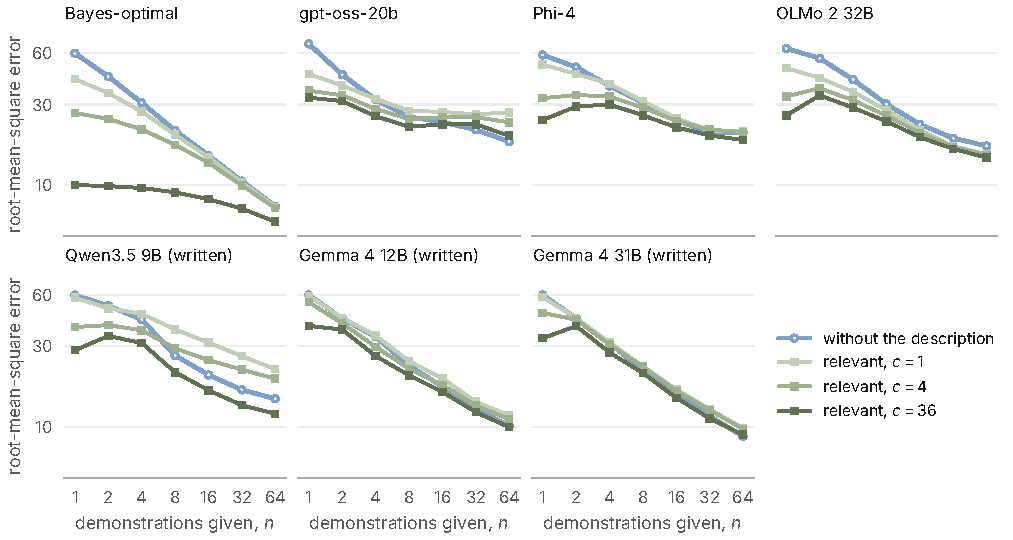
\includegraphics[width=\textwidth]{llm_curves.pdf}
\caption[Learning curves used to estimate language-model ESS]{\textbf{Learning curves used to estimate language-model ESS.} Root-mean-square error versus demonstration count for the reference and six models in the full run without reasoning, at $\sigma = 60$. Blue curves omit the description; green curves use relevant descriptions, with darker shades indicating higher $c$. Replies without a number are excluded. ESS is the horizontal distance from the description-conditioned point at $n$ to the baseline curve at the same error. For four models, error with $c = 36$ increases between one and two demonstrations because the models shift toward the observations more than the reference does (Table~\ref{tab:llm-full}).}
\label{fig:curves}
\end{figure}

\begin{table}[htbp]
\centering\small
\setlength{\tabcolsep}{4pt}
\caption[Sensitivity of summary ESS to baseline-curve estimation]{\textbf{Sensitivity of summary ESS to baseline-curve estimation.} Median ESS over $n = 1$, $2$, and $4$ for relevant descriptions, using the full run without reasoning at $\sigma = 60$. ``Log $n$'' is the primary estimator; ``linear'' interpolates in $n$; ``monotone'' applies a non-increasing fit; and ``fit'' uses $A/(n+n_0)+B$. The reference's idealized ESS values are $1$, $4$, and $36$.}
\label{tab:sensitivity}
\vspace{3pt}
\fittable{../../results/llm-test/llm_table_sensitivity.tex}
\end{table}

\section{Results of the Full Run}\label{sec:llm-full-run}

\paragraph{Summary ESS.}
Across the six models, the $c = 36$ description has summary ESS $1.4$ to $7.6$, compared with reference ESS $36$ on these tasks, and ESS at most $15$ at any of $n = 1$, $2$, and $4$ (Table~\ref{tab:llm}). The $c = 1$ and $c = 4$ descriptions have summary ESS $0.0$ to $1.9$ and $0.2$ to $4.1$, compared with $1.3$ and $4.4$. ESS rises with $c$ mainly because a more specific description has a value closer to the task, as Table~\ref{tab:control} shows.

\paragraph{Description weights.}
At $\sigma = 60$, with no demonstrations and no stated reliability, the models return the description value (weight $0.92$ to $1.10$), although Phi-4 and OLMo~2 32B then begin only $20$ to $23\%$ and $50$ to $59\%$ of their replies with a number. At $n = 1$, the weight of gpt-oss-20b, Phi-4, and OLMo~2 32B changes by at most $0.08$ from $c = 1$ to $c = 36$, and if anything falls, whereas the reference weight rises from $0.50$ to $0.80$ to $0.97$ (Table~\ref{tab:llm}). At every $n$ from $1$ to $64$ and at both noise levels, the spread of these three models' weights across $c$ is at most $0.16$, compared with a reference spread of $0.34$ to $0.71$ (Table~\ref{tab:llm-full}). The weights of the two Gemma models do rise with $c$, by about $0.25$ between $c = 1$ and $c = 36$ at $n = 1$, half the reference rise. The weight of Qwen3.5 9B does not. Models therefore underweight a precise description and, with many demonstrations, overweight the least precise one. At $n = 64$, gpt-oss-20b still assigns weight $0.23$ to the $c = 1$ value, compared with reference weight $0.02$, and that description raises its error (ESS $-57$).

\paragraph{Stated unreliability.}
A stated $10\%$ or $50\%$ chance of being wrong leaves the ESS of gpt-oss-20b and OLMo~2 32B about where it was, and Phi-4's ESS even rises, from $7.6$ to $8.7$ and $9.7$. Qwen3.5 9B and Gemma~4 31B have lower ESS, but by about as much for $50\%$ as for $10\%$. Gemma~4 12B's ESS falls at $10\%$ and rises at $50\%$ (Table~\ref{tab:llm}). No model's ESS falls in proportion to the stated probability, whereas reference ESS falls to $22$ and $5.8$.

\section{Unreliability, Description Accuracy, and Wording}\label{sec:llm-unreliability}

\paragraph{Irrelevant descriptions.}
An irrelevant description uses the value from a different, independently sampled task. At $c = 36$, these descriptions have negative ESS for every model and for the prompt-based reference, which treats them as relevant. The models assign less weight to the description and consequently incur lower error in this condition: at $n = 4$, their root-mean-square errors range from $35$ to $64$, compared with $124$ for the reference. Also at $n = 4$, their weight on an irrelevant $c = 36$ value is $0.01$ to $0.33$, compared with $0.18$ to $0.44$ on a relevant one.

\paragraph{Actual unreliability.}
The stated-unreliability experiments keep descriptions relevant and vary what models are told. Table~\ref{tab:mixture} instead evaluates the mixture in Chapter~\ref{ch:setup}. We combine squared errors from the relevant and irrelevant conditions, on the same tasks, with weights $p$ and $1-p$, and then estimate ESS. We evaluate models both with and without disclosure of the irrelevance probability. The fully trusting reference always treats the description as relevant; the calibrated reference starts from irrelevance probability $1-p$ and updates it from the observations.

At actual reliability $p = 0.9$, a $c = 36$ description has ESS $5.5$ for the calibrated reference and $0.2$ for the fully trusting reference. Model ESS ranges from $0.4$ to $3.2$ when the reliability is not stated and from $-0.1$ to $4.0$ when it is stated. Model weights depend weakly on $p$, and stating the probability changes ESS by at most two demonstrations in either direction. Their nearly fixed weight on the description thus acts as a hedge between full trust and calibration. At $p = 0.5$, the description is worth less than one demonstration to the calibrated reference and at most one to every model.

\begin{table}[htbp]
\caption[Description ESS under actual unreliability]{\textbf{Description ESS under actual unreliability.} Relevant and irrelevant $c = 36$ conditions are combined with weights $p$ and $1-p$. Results are summary ESS with $95\%$ task-bootstrap intervals for the full run without reasoning at $\sigma = 60$. The fully trusting reference assumes relevance; the calibrated reference uses the actual reliability and updates it from demonstrations. A bound indicates that one demonstration alone outperforms the description-conditioned prediction at one or more summary demonstration counts.}
\label{tab:mixture}
\centering\footnotesize
\fittable{../../results/llm-test/llm_table_mixture.tex}
\end{table}

\paragraph{Wording without reasoning.}
We repeat the three relevant-description conditions and the no-description baseline at $n = 1$, $2$, and $4$ using three alternative description sentences: ``Its mean is about $m$, give or take $\tau$.'', ``Mean: $m \pm \tau$'', and ``An earlier estimate put its mean at $m$, with a standard error of $\tau$.'' Table~\ref{tab:paraphrase} uses the full-run tasks and written readouts.

Wording substantially changes the weight assigned to the description. For Gemma~4 12B with $c = 1$ and $n = 1$, this weight is $0.34$ under the original wording and $1.00$ under each alternative. For gpt-oss-20b, it ranges from $0.17$ to $0.67$. A coefficient above $1$ means that predictions vary more strongly with the stated value than the value itself. Nevertheless, none of the tested wordings yields the reference's sensitivity to specificity: across models and wordings, the weight difference between $c = 36$ and $c = 1$ is at most $0.25$ at $n = 1$ and $0.44$ at $n = 4$, compared with reference differences of $0.47$ and $0.70$. The informal descriptions do not uniquely specify a probability distribution, so this comparison also varies how precisely the task is specified.

\begin{table}[htbp]
\centering\footnotesize
\caption[Description weights under four wordings without reasoning]{\textbf{Description weights under four wordings without reasoning.} Weights are reported for the three relevant descriptions at $n = 1$ and $4$, using written readouts on the full-run tasks. ``Number'' denotes the numeric response rate; italics mark rates below three quarters. The reference weights are $0.50$, $0.80$, and $0.97$ at $n = 1$, and $0.20$, $0.50$, and $0.90$ at $n = 4$. Wording changes overall reliance on the description, but the observed change with stated specificity remains smaller than the reference change.}
\label{tab:paraphrase}
\vspace{3pt}
\fittable{../../results/llm-test/llm_table_paraphrase.tex}
\end{table}

\paragraph{Separating stated specificity from description accuracy.}
For each task, we take a description value generated either at $c = 36$ or at $c = 1$ and present it with each stated specificity in $\{1,4,36\}$. The tasks and demonstrations match the full run, and the experiment includes its own no-description prompts at every $n$ (Table~\ref{tab:control}). Repeated conditions reproduce the full run exactly except for gpt-oss-20b. Its distribution readout changes by a median of $0.8$ to $1.2$ across conditions, with a maximum difference of $39$; its written replies change in $12\%$ of cases, with median difference $0$. A newer library version is a possible explanation.

The prompt-based reference accepts the stated specificity. A value generated at $c = 1$ but stated as $c = 36$ therefore has reference ESS of about $-0.8$; a model that discounts the stated specificity can outperform it in that misspecified condition. For models without reasoning, description accuracy primarily determines ESS. When the value is generated at $c = 1$, each model's ESS remains between $-0.1$ and $2.0$ across all stated specificities. When the value is generated at $c = 36$, each model's ESS is higher, but from stated $c = 1$ to stated $c = 36$ it rises by at most $1.2$, whereas reference ESS rises from $2.5$ to $36$. For example, gpt-oss-20b has ESS $2.7$, $2.6$, and $2.8$ at stated $c = 1$, $4$, and $36$. Phi-4's ESS even falls, from $12$ at stated $c = 1$ to $7.6$ at stated $c = 36$, the reverse of the reference order.

\begin{table}[htbp]
\centering\small
\setlength{\tabcolsep}{4pt}
\caption[Sensitivity to stated specificity with the value and demonstrations held fixed]{\textbf{Sensitivity to stated specificity with the value and demonstrations held fixed.} Results use $\sigma = 60$, the full-run tasks, and the readout conventions of Table~\ref{tab:llm}. For a value generated at $c = 36$, the table reports its weight at $n = 1$ and summary ESS under each stated $c$. Results for the $200$-task runs of Sections~\ref{sec:llm-task}--\ref{sec:llm-stated} appear in Table~\ref{tab:reason}.}
\label{tab:control}
\vspace{3pt}
\fittable{../../results/llm-test/control_table.tex}
\end{table}

\section{Reasoning Runs and Execution Settings}\label{sec:llm-runs}

\paragraph{Shared evaluation prompts.}
Every model in Figure~\ref{fig:llm}, as well as Olmo~3 7B Think \citep{olmo2025three}, is evaluated on the same $7{,}800$ prompts from the first $200$ tasks. These include no-description prompts at $n = 1$, $2$, $4$, $\ldots$, $64$, with additional points at $n = 40$ and $48$ near the $c = 36$ crossing, and every description condition at $n = 1$, $2$, and $4$. The gpt-oss-20b run omits the two additional points and contains $7{,}400$ prompts. Results without reasoning for the open-weight models are taken from the full run restricted to these tasks. The two modes receive the same prompts, although their serving environments can differ as detailed below. At least $99.7\%$ of replies in each run contain a number.

\paragraph{Open-weight reasoning models.}
With reasoning, gpt-oss-20b runs in vLLM using greedy decoding, low reasoning effort, and at most $4{,}096$ new tokens. It reaches the final channel in $99.9\%$ of replies and uses $322$ tokens on average, and at least $97\%$ of replies reach it in every cell. An earlier run with a limit of $384$ tokens finished only $28$ to $54\%$ of the replies in the stated-reliability conditions, and the difference between a stated $10\%$ and $50\%$ that this run seemed to show came from which replies finished. Qwen3.5 9B runs through OpenRouter at temperature $0$, with reasoning enabled and a limit of $24{,}576$ new tokens. We pin requests to DeepInfra, which serves the model in bf16, because quantization varies across providers. Of its replies, $2{,}305$ loop to the token limit, a failure its model card warns of. Each is rerun once using the model card's recommended reasoning sampling settings (temperature $1.0$, top-$p$ $0.95$, top-$k$ $20$, presence penalty $1.5$); $10$ remain unfinished.

Gemma~4 31B (\texttt{gemma-4-31b-it}) runs through the Gemini API at temperature $0$. Reasoning is enabled by default, and the model uses $2{,}613$ reasoning tokens on average, with the same $24{,}576$-token limit. Of its replies, $435$ reach the limit; all finish after one rerun using the model card's recommended sampling settings (temperature $1.0$, top-$p$ $0.95$, top-$k$ $64$).

Olmo~3 7B Think runs in vLLM with greedy decoding and at most $32{,}768$ new tokens, the limit its model card recommends; at $8{,}192$ tokens, only $12$ of $20$ pilot replies finished. We rerun the $169$ replies that reach this limit once with temperature $0.6$ and top-$p$ $0.95$; $17$ remain unfinished. The model uses $9{,}215$ reasoning tokens on average. Its long greedy outputs are sensitive to hardware: an earlier stated-specificity run on a different GPU produces the same final number on only half the prompts. We therefore report one run. Despite its extensive reasoning, this model learns little from the demonstrations; its prediction behavior is reported below.

\paragraph{Models served through command-line agents.}
GPT-6 Sol (\texttt{gpt-6-sol}) runs through the Codex command-line agent under a subscription, in a read-only sandbox. We evaluate reasoning disabled, with no reasoning tokens, and reasoning enabled at low effort. The agent's instructions and tool definitions surround the prompt, much as a provider's system prompt surrounds a prompt sent through an API. The model invokes a shell command in $544$ replies with reasoning and $616$ without reasoning. Almost all such calls average demonstrations in no-description prompts with at least eight observations; other prompts account for seven calls with reasoning and $97$ without it. Improving the baseline error curve through these calculations lowers the ESS inferred from that curve. Tool use therefore does not inflate ESS through a weaker baseline, although access to tools remains a difference between this execution environment and tool-free runs.

Claude Opus~4.6 and Haiku~5.5 run through the Claude Code command line under a subscription, with one prompt per call, no tools, no project or user instructions, and a one-line system prompt. Opus~4.6 uses high effort in both evaluated modes, with reasoning either enabled or disabled; the disabled mode emits no reasoning tokens. When enabled, it reasons before at least $99\%$ of replies in each description condition and averages $599$ reasoning tokens across all replies. Without a description, it reasons before only $1\%$, $24\%$, and $79\%$ of replies at $n = 1$, $2$, and $4$, respectively. Haiku~5.5 (\texttt{claude-haiku-5-5}) is evaluated at medium and low effort, using the command line's default sampling temperature. At medium effort, it reasons before $37$ to $88\%$ of replies at $n = 1$ across conditions and before nearly all replies from $n = 2$ onward, with $270$ reasoning tokens on average. Its no-description error stays close to the reference through $n = 48$; at $n = 16$, for example, it is $15.8$ against $14.8$, with two replies far off. Its error rises at $n = 64$, where it divides the sum by $60$ instead of $64$ in $9$ of $200$ replies.

\paragraph{Interpreting the comparison between modes.}
The experiments hold the model checkpoint and prompts fixed within each paired comparison, but reasoning settings, serving software, readout, retry policy, and access to calculation tools are not uniform across all runs. The results describe the behavior of the evaluated configurations. They do not by themselves isolate a single internal mechanism responsible for the difference between modes.

\paragraph{ESS when baseline arithmetic fails.}
With reasoning, gpt-oss-20b and Qwen3.5 9B assign approximately the reference weight to the description: at $n = 4$ and $c = 36$, their weights are $0.89$ and $0.90$, compared with $0.90$ for the reference. However, both make errors when averaging longer demonstration sequences. Qwen3.5 9B has no-description root-mean-square error $15.1$ at $n = 16$ and $35.4$ at $n = 32$, compared with reference errors $14.8$ and $10.0$. From $n = 32$ onward, between $4$ and $24$ replies per cell differ from the sample mean by more than $20$; one reply gives $945$ for numbers averaging $467$.

For these models, the baseline curve rises after $16$ demonstrations, and some description-conditioned errors never meet it within the evaluated grid. Table~\ref{tab:reason} therefore also reports, in parentheses, a comparison using the Bayesian reference's baseline curve. This quantity is the number of demonstrations required by the reference without a description to match the model's error, rather than ESS in the model's own units. The gpt-oss-20b model also makes arithmetic errors with descriptions, reducing the reported ESS in those conditions; for example, it obtains $1.3$ when the prompt states a $10\%$ chance of being wrong. About $2\%$ of its replies are more than $40$ from the reference prediction, from errors such as exchanging the two variances. On the reference's baseline, its $c = 36$ description is therefore worth $24$ demonstrations, well below the reference's $34.6$, although its weight is right. A fitted weight hides such errors, whereas ESS does not.

Opus~4.6 and GPT-6 Sol do not exhibit these arithmetic failures. Opus~4.6 has root-mean-square error $7.4$ at $n = 64$, matching the reference on these tasks, and using either baseline gives the same ESS for these two models. At low effort, Haiku~5.5 often skips reasoning and repeats the demonstration. Its description weight at $n = 1$ is consequently low even in conditions whose ESS is close to the reference value.

\begin{table}[htbp]
\centering\small
\setlength{\tabcolsep}{2.5pt}
\caption[Description ESS across reasoning configurations]{\textbf{Description ESS across reasoning configurations.} Results use the first $200$ tasks at $\sigma = 60$. Summary ESS is computed using each run's baseline curve; parentheses show the value using the Bayesian reference's baseline where it differs. ``10\% wrong'' and ``50\% wrong'' denote the stated probability for a $c = 36$ description. The last column uses a value generated at $c = 36$ but described as $c = 4$. ``Reasoning'' identifies the mode and provider effort setting. An upper bound, $\leq$, indicates that one demonstration alone gives lower error; $>60$ denotes a crossing beyond the grid. Reference values use the same tasks and estimator. Olmo~3 7B Think's no-description error never drops below its error at one demonstration, so its reported crossings require particular caution; using the reference baseline gives a different comparison rather than resolving the weak model baseline.}
\label{tab:reason}
\vspace{3pt}
\fittable{../paper/tables/reason_table.tex}
\end{table}

\section{Prediction Rules and Reliability Updating}\label{sec:llm-rules}

\paragraph{Rules inferred from individual replies.}
A weight fitted across tasks can mix replies that follow different rules. At $n = 4$, we estimate the description weight implied by an individual prediction as $(\hat y-\bar y)/(m-\bar y)$. We use the $61$ tasks per cell where $|m-\bar y|\geq30$ and exclude replies without a number. We classify a reply as consistent with a rule if its implied weight is within $0.05$ of that rule's weight. The candidate weights are the Bayesian reference ($0.90$ for $c = 36$ and $0.20$ for $c = 1$); the reference with its two precisions exchanged ($0.10$ and $0.80$); the description counted as one additional observation, $1/(n+1)$; the description alone, with weight $1$; and the demonstrations alone, with weight $0$. The one-additional-observation rule coincides with the reference at $c = 1$.

With reasoning, Opus~4.6, GPT-6 Sol, Gemma~4 31B, and Haiku~5.5 match the reference rule on $95$ to $100\%$ of eligible replies. Without reasoning, $79\%$ of Opus~4.6 replies at $c = 36$ match none of these candidate rules, as do more than half of GPT-6 Sol replies. Olmo~3 7B Think instead repeats the description value in $96$ to $97\%$ of replies at $n = 1$, regardless of stated specificity. At $n = 4$, $70$ to $77\%$ of its replies match none of the rules, and only $3$ to $8\%$ match the reference. From task to task, it predicts the description value, the demonstration mean, or an invented pattern, and it makes arithmetic errors. Its no-description root-mean-square error remains near $55$ from $n = 1$ to $32$, compared with reference error $10$ at $n = 32$. Reasoning mode is therefore not sufficient for the desired behavior in every tested model.

Within each cell, Haiku~5.5's replies split by whether it reasons. At $n = 1$, replies with reasoning assign weights $0.50$, $0.80$, and $0.97$ to the relevant $c = 1$, $4$, and $36$ values, the reference weights to two decimals, at either effort. Replies without reasoning assign weight $0.00$ to $0.05$ and repeat the demonstration. Its overall weight at $n = 1$ mixes the two kinds of reply: $0.44$, $0.66$, and $0.74$ at medium effort. On these three descriptions, it reasons before $34$ to $53\%$ of replies at low effort, against $72$ to $82\%$ at medium effort, so its overall weight at $n = 1$ is lower at low effort and nearly flat, at $0.36$, $0.34$, and $0.41$. With more demonstrations it reasons more often, and its weight approaches the reference again: at $n = 4$ and low effort, it is $0.17$, $0.48$, and $0.86$, compared with $0.20$, $0.50$, and $0.90$. The choice to reason is the model's own, so this split describes its replies rather than the result of an experiment.

\paragraph{A fixed reliability rule.}
Table~\ref{tab:hedge} reports description weights for $c = 36$ when the prompt states a probability of being wrong. A predictor that combines the description-conditioned and no-description predictions with fixed weights $p$ and $1-p$ assigns weight $p\,36/(36+n)$ to $m$. Under the original warning, which leaves the fallback unstated, GPT-6 Sol, Gemma~4 31B, and Qwen3.5 9B with reasoning are close to this fixed rule. Opus~4.6 and Haiku~5.5 at medium effort fall below the reference weight by $n = 4$. Haiku~5.5 at low effort, which often skips reasoning at $n = 1$, comes closest to the reference weight. gpt-oss-20b assigns nearly the weight of a reliable description whatever the stated probability. These are behavioral comparisons; they do not identify the internal procedure used in every reply.

\paragraph{Sensitivity to the unspecified fallback prior.}
The prompt states only that, if the description is wrong, ``the mean is unknown''. A Bayesian relevance update compares the likelihood of the observations under the description with their likelihood under this fallback. Because the prompt leaves the fallback distribution unspecified, it does not determine a unique Bayesian relevance update.

For the $c = 36$ description with a stated $50\%$ chance of being wrong, the reference's fitted weights on the first $200$ tasks at $n = 1$, $2$, $4$, $8$, and $16$ are $0.58$, $0.61$, $0.64$, $0.58$, and $0.54$ with the uniform fallback over $100$ to $999$. They are $0.49$, $0.49$, $0.53$, $0.49$, and $0.45$ with the actual task prior $\mathcal{N}(500,100^2)$; $0.52$, $0.54$, $0.58$, $0.53$, and $0.49$ with $\mathcal{N}(500,200^2)$; and $0.72$, $0.74$, $0.74$, $0.67$, and $0.60$ with a uniform fallback over $0$ to $2{,}000$. The fixed rule gives $0.49$, $0.47$, $0.45$, $0.41$, and $0.35$.

By four demonstrations, the reference weight exceeds the fixed-rule weight for every fallback examined. Thus the observed agreement of several models with the fixed rule persists across these choices of reference. The size of their departure from Bayesian updating depends on the fallback, however; under the actual task prior, the reference update is small before four demonstrations.

\begin{table}[htbp]
\centering\small
\setlength{\tabcolsep}{3pt}
\caption[Description weights under stated unreliability]{\textbf{Description weights under stated unreliability.} Coefficients on the $c = 36$ description value for the first $200$ tasks, with stated irrelevance probability $1-p$. ``Fixed'' uses weight $p\,36/(36+n)$; the reference updates relevance using the uniform fallback over $100$ to $999$. Bootstrap standard errors are at most $0.03$ at $n = 4$ in the stated-$50\%$ condition, and at most $0.06$ overall, except for gpt-oss-20b, whose maximum is $0.09$. Several reasoning configurations closely track the fixed rule.}
\label{tab:hedge}
\vspace{3pt}
\begin{tabular}{lcccccc}
\toprule
& \multicolumn{3}{c}{$50\%$ wrong} & \multicolumn{3}{c}{$10\%$ wrong} \\
\cmidrule(lr){2-4} \cmidrule(lr){5-7}
& $n = 1$ & $2$ & $4$ & $1$ & $2$ & $4$ \\
\midrule
Reference & $0.58$ & $0.61$ & $0.64$ & $0.88$ & $0.87$ & $0.84$ \\
Fixed & $0.49$ & $0.47$ & $0.45$ & $0.88$ & $0.85$ & $0.81$ \\
\midrule
GPT-6 Sol & $0.50$ & $0.48$ & $0.45$ & $0.92$ & $0.88$ & $0.82$ \\
Opus~4.6 & $0.56$ & $0.43$ & $0.40$ & $0.93$ & $0.86$ & $0.77$ \\
Gemma~4 31B & $0.49$ & $0.46$ & $0.45$ & $0.89$ & $0.68$ & $0.76$ \\
Qwen3.5 9B & $0.50$ & $0.46$ & $0.43$ & $0.88$ & $0.84$ & $0.74$ \\
Haiku~5.5, medium & $0.55$ & $0.56$ & $0.46$ & $0.79$ & $0.93$ & $0.89$ \\
Haiku~5.5, low & $0.49$ & $0.62$ & $0.58$ & $0.42$ & $0.94$ & $0.88$ \\
gpt-oss-20b & $0.89$ & $0.87$ & $0.82$ & $0.95$ & $0.87$ & $0.90$ \\
\bottomrule
\end{tabular}
\end{table}

\paragraph{Stating the fallback.}
To remove this ambiguity, we rerun the stated-reliability condition on the same $200$ tasks, for $c = 36$, stated chances of $10\%$ and $50\%$, and $n = 1$, $2$, $4$, with the fallback stated as the reference's uniform over $100$ to $999$. We use GPT-6 Sol at low effort and Haiku~5.5 at medium effort, with $1{,}200$ prompts each. Table~\ref{tab:fallback} compares their description weights with those of the original runs. With a stated $50\%$ chance, the reference and the fixed rule differ by at least $5$ on $123$ to $155$ tasks per cell. On those tasks, the share of replies closer to the reference than to the fixed rule rises from $0$--$2\%$ to $89$--$97\%$ for GPT-6 Sol and from $21$--$41\%$ to $87$--$95\%$ for Haiku~5.5. With a stated $10\%$ chance, at most $7$ tasks per cell separate the two rules, so this share is uninformative there.

Summary ESS, computed against each model's original curve without the description, barely moves at $50\%$: from $4.4$ to $4.7$ for GPT-6 Sol and from $3.8$ to $4.2$ for Haiku~5.5, against $5.7$ for the reference, because the two rules give similar errors at $n \le 4$. At $10\%$, it falls from $30.3$ to $17.8$ and from $32.6$ to $17.9$, against $27.5$: with the fallback stated, the models discount the description more than the reference does.

\begin{table}[htbp]
\centering\small
\setlength{\tabcolsep}{3pt}
\caption[Stating the fallback changes the reliability rule]{\textbf{Stating the fallback changes the reliability rule.} Coefficients on the $c = 36$ description value for the first $200$ tasks, as in Table~\ref{tab:hedge}. ``Unstated'': the original warning, ``the mean is unknown''; ``stated'': the mean is otherwise uniform over $100$ to $999$, as the reference assumes.}
\label{tab:fallback}
\vspace{3pt}
\begin{tabular}{lcccccc}
\toprule
& \multicolumn{3}{c}{$50\%$ wrong} & \multicolumn{3}{c}{$10\%$ wrong} \\
\cmidrule(lr){2-4} \cmidrule(lr){5-7}
& $n = 1$ & $2$ & $4$ & $1$ & $2$ & $4$ \\
\midrule
Reference & $0.58$ & $0.61$ & $0.64$ & $0.88$ & $0.87$ & $0.84$ \\
Fixed & $0.49$ & $0.47$ & $0.45$ & $0.88$ & $0.85$ & $0.81$ \\
\midrule
GPT-6 Sol, unstated & $0.50$ & $0.48$ & $0.45$ & $0.92$ & $0.88$ & $0.82$ \\
GPT-6 Sol, stated & $0.57$ & $0.58$ & $0.58$ & $0.86$ & $0.82$ & $0.75$ \\
Haiku~5.5, unstated & $0.55$ & $0.56$ & $0.46$ & $0.79$ & $0.93$ & $0.89$ \\
Haiku~5.5, stated & $0.62$ & $0.60$ & $0.63$ & $0.89$ & $0.84$ & $0.80$ \\
\bottomrule
\end{tabular}
\end{table}

\section{Wording with Reasoning Enabled}

\paragraph{GPT-6 Sol.}
We evaluate the three alternative wordings at low effort for the three relevant descriptions and $n = 1$, $2$, and $4$, using the first $200$ tasks. Of $5{,}400$ replies, $5{,}399$ contain a number. Under ``An earlier estimate put its mean at $m$, with a standard error of $\tau$'', the model reasons before every reply, and its description weight is within $0.01$ of the reference in every cell, as under the original wording.

Under ``Its mean is about $m$, give or take $\tau$'' and ``Mean: $m \pm \tau$'', it skips reasoning in $24$ to $51\%$ and $11$ to $50\%$ of replies per cell, respectively. Of those replies, $83\%$ and $87\%$ repeat the description value. At $c = 1$ and $n = 1$, the fitted description weights are consequently $0.89$ and $1.00$, compared with reference weight $0.50$. Among replies that do include reasoning, $68\%$ and $43\%$ are within $1$ of the reference prediction, while $36\%$ and $68\%$ repeat the description value. These categories overlap at $c = 36$, where the description value and reference prediction can be close. Under any reading of $\tau$, the reference prediction moves with the demonstrations, yet most replies that skip reasoning repeat the description value.

\paragraph{Haiku~5.5.}
We evaluate the same alternatives at medium effort; all $5{,}400$ replies contain a number. Under ``An earlier estimate put its mean at $m$, with a standard error of $\tau$'', the model reasons before at least $72\%$ of replies in each cell, and $99\%$ of the replies with reasoning lie within $1$ of the reference prediction. Under ``Its mean is about $m$, give or take $\tau$'' and ``Mean: $m \pm \tau$'', it skips reasoning in $4$ to $36\%$ and $2$ to $74\%$ of replies per cell, respectively. Even among replies with reasoning, $71\%$ and $91\%$ repeat the description value, while $31\%$ and $20\%$ lie within $1$ of the reference prediction. At $c = 1$ and $n = 4$, its description weights are $0.72$ and $0.93$, compared with reference weight $0.20$.

These wording changes affect the precision of the probabilistic specification as well as the model's behavior. All provide a value $m$ and a scale $\tau$, but ``give or take'' and ``$\pm$'' do not uniquely identify $\tau$ as a prior standard deviation or establish a sampling model. The experiment therefore shows that accurate combination of descriptions and demonstrations under explicit statistical statements does not automatically transfer to these less explicit formulations. It does not isolate sensitivity to semantically equivalent descriptions.
